\section{RESULTADOS}

Apresentamos os resultados obtidos na comparação de diferentes modelos de aprendizado profundo na segmentação de feridas malignas em imagens médicas. Primeiramente, descrevemos o processo de criação do conjunto de dados clínicos e as técnicas de pré-processamento de imagens utilizadas. Em seguida, apresentamos os resultados de desempenho dos modelos, levando em consideração os resultados das métricas abordadas. Também realizamos uma análise comparativa entre os modelos e discutimos suas contribuições e perspectivas futuras. Esperamos que esses resultados possam contribuir para o desenvolvimento de ferramentas de diagnóstico e tratamento mais precisas e eficazes para pacientes com feridas malignas.

\subsection{Criação de um Dataset}
A criação de um dataset novo teve como principal finalidade assegurar a excelência e a confiabilidade dos dados, além da representatividade e diversidade das imagens. Imagens de lesões malignas foram meticulosamente coletadas de várias fontes, como repositórios públicos no GitHub e plataformas especializadas em imagens médicas. Selecionou-se um conjunto heterogêneo de mais de 4.500 imagens, representando variados tipos de lesões, tamanhos, formas e condições. Este procedimento prévio ao treinamento dos modelos assegura dados de alta qualidade e confiabilidade. Especificações detalhadas das imagens, incluindo resolução, dimensões e formato, foram definidas para proporcionar uma compreensão abrangente do dataset.

Os resultados obtidos com este dataset único para segmentação de lesões malignas sublinham sua importância vital no estudo. A qualidade e a confiabilidade são reforçadas pela coleta criteriosa, pré-processamento e anotação, junto com informações clínicas precisas, tornando estes dados recursos valiosos para os profissionais de saúde. A ampla gama de lesões capturadas garante que os modelos desenvolvidos sejam capazes de enfrentar a variedade encontrada em cenários clínicos reais. Uma distribuição equilibrada nas fases de treino e teste é crucial para uma avaliação correta do desempenho dos modelos, contribuindo para a generalização em diferentes casos clínicos. Este dataset robusto serve como um alicerce para desenvolver e testar modelos de segmentação de lesões malignas baseados em aprendizado profundo, elevando as possibilidades de análise precisa e abrangente das técnicas de segmentação propostas. A amplitude e diversidade deste dataset são determinantes para melhorar os resultados e efetivar modelos de aprendizado profundo na segmentação de lesões malignas.

\subsection{Desempenho dos Modelos}

    % Os modelos de aprendizagem profunda deverão ser capazes de segmentar com sucesso as feridas malignas nas imagens médicas. A performance de cada modelo será avaliada utilizando métricas como acurácia, precisão, recall, F1-score e coeficiente de Dice.
    
    % Espera-se que todos os modelos apresentem bom desempenho, dada a capacidade das arquiteturas escolhidas para a tarefa de segmentação de imagem. Contudo, algumas diferenças no desempenho podem ocorrer devido às características específicas de cada arquitetura.
    
Este estudo avaliou a eficácia de modelos de aprendizado profundo, especificamente \ac{FCN}, \ac{U-Net}, \ac{SegNet} e \ac{MobileNetV2}, na segmentação de feridas malignas em imagens médicas. A metodologia proposta gerou resultados significativos.
    
\subsubsection{FCN}
Após 150 épocas de treinamento, o modelo \ac{FCN} demonstrou eficácia notável na segmentação de pixels em imagens médicas. A Figura~\ref{fig:graphFCN} abaixo, ilustra que a \textit{Loss} do modelo começa ligeiramente acima de zero, mantendo-se estável ao longo das épocas, o que evidencia um aprendizado consistente. No entanto, os picos observados nos valores de \textit{test loss} em torno das 100 e 150 épocas indicam desafios na generalização do modelo para novos dados.

\begin{figure}[htbp]
    \centering
    \caption{Gráfico do Treinamento do Modelo \acf{FCN}}
    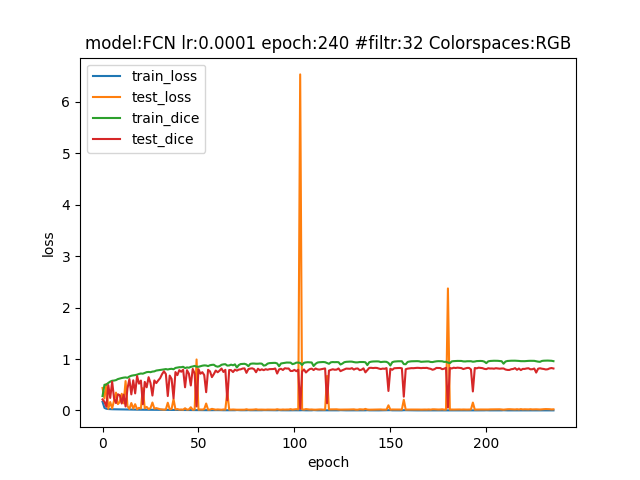
\includegraphics[width=0.9\textwidth]{img/fcnmodelfile.png}
    \label{fig:graphFCN}
    \par\medskip\textbf{Fonte:} Autor
\end{figure}

Os indicadores principais de desempenho do \ac{FCN} incluem:

\textbf{Precision:} O modelo atingiu uma precisão de 0,9737, identificando acertadamente cerca de 97,37\% dos pixels em áreas de feridas malignas, evidenciando sua alta precisão na segmentação correta desses pixels.

\textbf{Recall:} Com um recall de 0,9527, o \ac{FCN} conseguiu detectar aproximadamente 95,27\% dos pixels efetivamente pertencentes a feridas malignas, destacando sua capacidade de identificar a maioria das áreas relevantes com mínima omissão.

\textbf{Coeficiente Dice:} O Coeficiente Dice alcançou 95,87\%, mostrando alta concordância entre a segmentação realizada pelo modelo e a manual, indicando uma sobreposição significativa entre as áreas identificadas pelo modelo e as marcadas manualmente.

Como evidenciado na Figura~\ref{fig:graphFCN}, o valor do \textit{train dice} permanece próximo a 1 durante o treinamento, refletindo uma excelente concordância entre a segmentação do modelo e a manual. A variação inicial do \textit{test dice} seguida por uma estabilização nas primeiras 60 épocas sinaliza um período de aprendizado inicial e subsequente aumento na estabilidade. Esses resultados sublinham a competência do \ac{FCN} em identificar e segmentar com precisão áreas afetadas em imagens médicas de feridas malignas, fornecendo uma base confiável para diagnóstico e tratamento.

\subsubsection{U-Net}
A Figura~\ref{fig:graphU-Net}, exibida abaixo, mostra a evolução das métricas de \textit{train loss}, \textit{test loss}, \textit{train dice} e \textit{test dice} no treinamento do modelo \ac{U-Net}. Inicialmente, tanto o \textit{train loss} quanto o \textit{test loss} começam ligeiramente acima de zero e rapidamente diminuem, apresentando um pico notável em torno das 35 épocas. Após este pico, os valores se estabilizam próximos a zero, indicando um aprendizado eficiente dos padrões nas imagens de feridas malignas com baixa perda.

\begin{figure}[htbp]
    \centering
    \caption{Gráfico do Treinamento do Modelo \acf{U-Net}}
    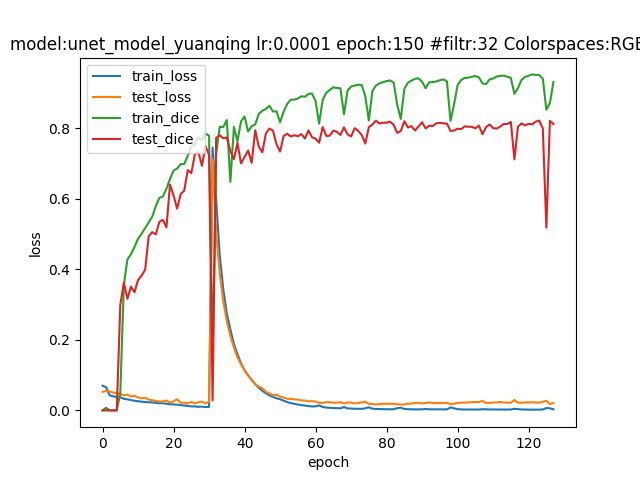
\includegraphics[width=0.8\textwidth]{img/unetprunedmodelfile.png}
    \label{fig:graphU-Net}
    \par\medskip\textbf{Fonte:} Autor
\end{figure}

O \ac{U-Net}, aplicado à segmentação de feridas malignas, mostrou resultados altamente promissores. Após 150 épocas, comparativamente ao \ac{FCN}, o modelo alcançou:

\textbf{Precisão (Precision):} Com uma precisão de 0,9471, o \ac{U-Net} identificou corretamente aproximadamente 94,71\% dos pixels em áreas de feridas malignas, um indicativo crucial para a identificação precisa em imagens médicas.

\textbf{Recall:} O modelo atingiu um recall de 0,9222, capturando cerca de 92,22\% dos pixels verdadeiramente pertencentes a feridas malignas, minimizando a omissão de áreas relevantes.

\textbf{Coeficiente Dice:} Com um valor de 93,07\%, o coeficiente Dice mostra a alta semelhança entre a segmentação prevista pelo modelo e a segmentação manual, indicando uma excelente concordância entre as duas.

Estes resultados evidenciam a robustez do \ac{U-Net} na identificação precisa de áreas de interesse em imagens médicas. O \textit{train dice}, conforme ilustrado na Figura~\ref{fig:graphU-Net} acima, começa em zero e rapidamente aumenta, estabilizando-se após cerca de 50 épocas. Isso sugere um aprendizado estável e consistente na sobreposição entre a segmentação do modelo e a manual. O \textit{test dice} exibe um comportamento semelhante, indicando boa generalização para dados novos, apesar de ligeiramente inferior. Tais achados ressaltam a capacidade notável do \ac{U-Net} em identificar com precisão as regiões de interesse nas imagens médicas de feridas malignas, proporcionando desempenho consistente e confiável para aplicações clínicas.

\subsubsection{SegNet}

A Figura~\ref{fig:graphSegNet} apresenta a evolução das métricas de \textit{train loss}, \textit{test loss}, \textit{train dice} e \textit{test dice} ao longo do treinamento do modelo \ac{SegNet}. 

\begin{figure}[htbp]
    \centering
    \caption{Gráfico do Treinamento do Modelo \acf{SegNet}}
    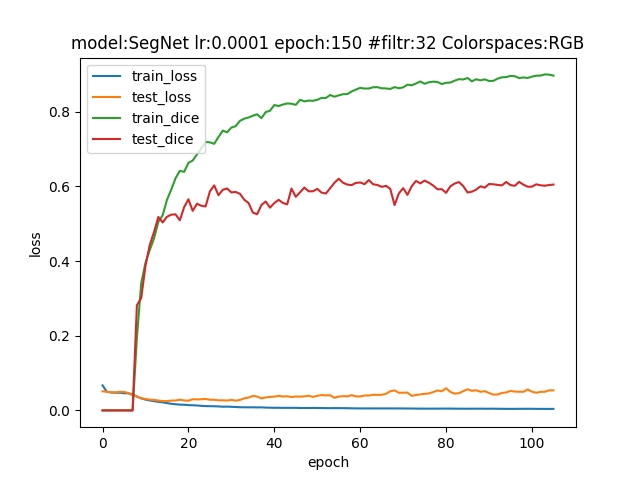
\includegraphics[width=0.7\textwidth]{img/segnetprunedmodelfile.png}
    \label{fig:graphSegNet}
    \par\medskip\textbf{Fonte:} Autor
\end{figure}

Observa-se uma estabilização nessas métricas após determinado número de épocas, indicando a convergência e a consolidação do desempenho do modelo. Esta estabilização reflete o aprendizado efetivo do \ac{SegNet} nos padrões necessários para a segmentação de feridas malignas, apesar de suas métricas serem levemente inferiores às de outros modelos. O desempenho do \ac{SegNet} na segmentação de feridas malignas, embora ligeiramente inferior ao dos modelos \ac{U-Net} e \ac{FCN}, ainda é notável. As métricas de desempenho do \ac{SegNet} destacam aspectos importantes da sua eficácia:

\textbf{Precisão (Precision):} O \ac{SegNet} alcançou uma precisão de 0,9247, classificando corretamente cerca de 92,47\% dos pixels em áreas de feridas malignas. Esta métrica demonstra a habilidade do modelo em identificar com precisão as áreas de interesse.

\textbf{Recall:} Com um recall de 0,8787, o modelo identificou aproximadamente 87,87\% dos pixels verdadeiramente pertencentes às feridas malignas. Este resultado evidencia a capacidade do \ac{SegNet} de capturar a maioria das áreas relevantes.

\textbf{Coeficiente Dice:} O modelo atingiu um Coeficiente Dice de 89,64\%, indicando uma boa concordância entre a segmentação realizada pelo modelo e a segmentação manual. Este valor reflete a eficácia do \ac{SegNet} em termos de precisão e recall.

Conforme ilustrado na Figura~\ref{fig:graphSegNet} acima, o \ac{SegNet} emerge como uma alternativa viável para a segmentação de feridas malignas, particularmente em cenários com restrições computacionais ou outros fatores limitantes na seleção de modelos.
         
\subsubsection{MobileNetV2}
A Figura~\ref{fig:graphMobileNetV2} abaixo, exibe a trajetória das métricas de treinamento do \ac{MobileNetV2}. 

\begin{figure}[htbp]
    \centering
    \caption{Gráfico do Treinamento do Modelo \acf{MobileNetV2}}
    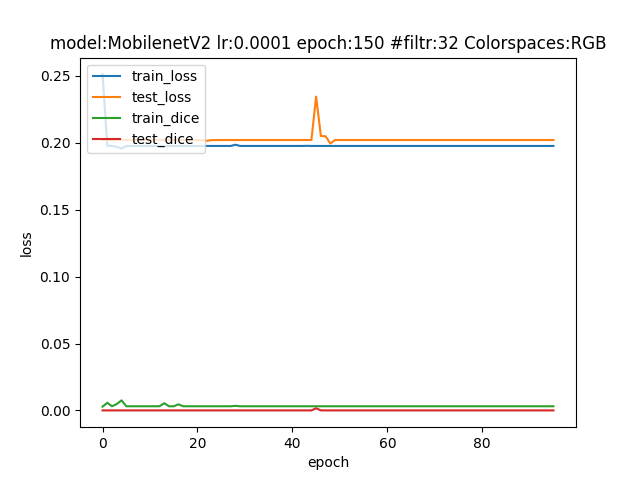
\includegraphics[width=0.7\textwidth]{img/mobilenetv2prunedmodelfile.png}
    \label{fig:graphMobileNetV2}
    \par\medskip\textbf{Fonte:} Autor
\end{figure}

A elevação significativa dos valores de \textit{loss} e a variação acentuada das métricas de desempenho ao longo do treinamento sinalizam uma instabilidade no aprendizado do modelo. No contexto da segmentação de feridas malignas, o \ac{MobileNetV2} exibiu desempenho consideravelmente inferior aos outros modelos testados. As métricas de desempenho evidenciam as deficiências deste modelo:

\textbf{Precisão (Precision):} O MobileNetV2 atingiu uma precisão de apenas 73,09\%, um valor significativamente menor em comparação aos demais modelos. Este resultado ressalta a dificuldade do modelo em identificar com precisão as áreas de interesse.

\textbf{Recall:} O modelo apresentou um recall de 62,19\%, detectando apenas cerca de 62,19\% dos pixels verdadeiramente associados a feridas malignas. Este resultado sublinha a limitação do modelo em capturar as áreas relevantes.

\textbf{Coeficiente Dice:} O MobileNetV2 registrou um Coeficiente Dice de apenas 62,61\%, indicando baixa concordância entre a segmentação efetuada pelo modelo e a segmentação manual. Este coeficiente reflete a ineficácia do modelo em termos de precisão e recall.

Como ilustrado na Figura~\ref{fig:graphMobileNetV2} acima, os resultados alcançados pelo \ac{MobileNetV2} são substancialmente inferiores aos dos outros modelos, evidenciando sua inadequação para a tarefa específica de segmentação de feridas malignas em imagens médicas. Essa análise aponta para a necessidade de desenvolvimento de modelos mais robustos para essa aplicação específica.

\subsection{Análise Comparativa Entre os Modelos}
Na Figura~\ref{fig:graphResultsModels} abaixo, apresentamos um gráfico comparativo que evidencia as métricas de precisão, recall e coeficiente Dice superiores do \ac{FCN} em relação aos outros modelos. 

\begin{figure}[htbp]
    \centering
    \caption{Comparação das Métricas dos Modelos Avaliados}
    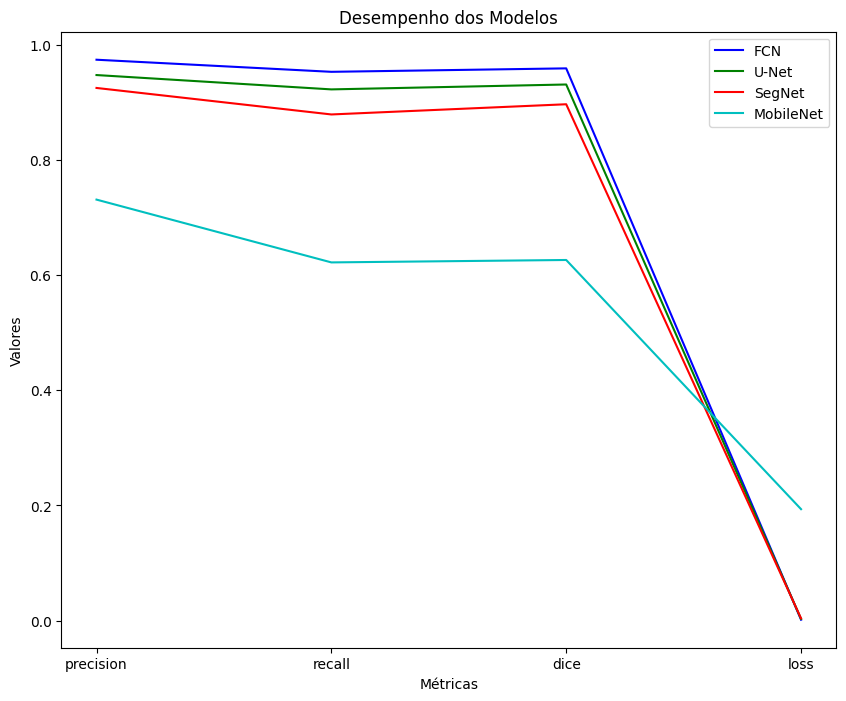
\includegraphics[width=0.7\textwidth]{img/results_metrics_models.png}
    \label{fig:graphResultsModels}
    \par\medskip\textbf{Fonte:} Autor
\end{figure}

Isso demonstra a excelência do \ac{FCN} em segmentação, complementada pela menor métrica de loss, indicativa de um erro reduzido na segmentação de feridas malignas.
\clearpage

A tabela \ref{tab:analiseMetricas} abaixo, mostra análise Comparativa das Métricas dos Modelos Avaliados \ac{FCN}, \ac{U-Net}, \ac{SegNet} e \ac{MobileNetV2}.  

\begin{table}[htbp]
    \centering
    \caption{Análise Comparativa das Métricas dos Modelos Avaliados}
    \begin{tabular}{|l|l|l|l|l|l|}
        \hline
        Modelos           & Epochs & Precision & Recall  & Dice    & Loss    \\ \hline
        \ac{FCN}          & 150    & 0.9737    & 0.9527  & 0.9687  & 0.0017  \\ \hline
        \ac{U-Net}        & 150    & 0.9471    & 0.9222  & 0.9307  & 0.0030  \\ \hline
        \ac{SegNet}       & 150    & 0.9247    & 0.8787  & 0.8964  & 0.0040  \\ \hline
        \ac{MobileNetV2}  & 150    & 0.7309    & 0.6219  & 0.6261  & 0.1936  \\ \hline
    \end{tabular}
    \label{tab:analiseMetricas}
    \par\medskip\textbf{Fonte:} Autor
\end{table}


%Podemos verificar a segmentação dos modelos nesta representação na figura \ref{fig:resultSegmetationModels} abaixo:
Na Figura~\ref{fig:resultSegmetationModels} abaixo, apresentamos exemplos de segmentações realizadas por cada modelo em nossa base de dados, destacando a superioridade do \ac{FCN} em termos de precisão. Enquanto \ac{U-Net} e \ac{SegNet} também mostram eficácia, o \ac{MobileNetV2} revela desempenho insatisfatório para esta tarefa específica.

\begin{figure}[htbp]
    \centering
    \caption{Resultado da Segmentação dos Modelos}
    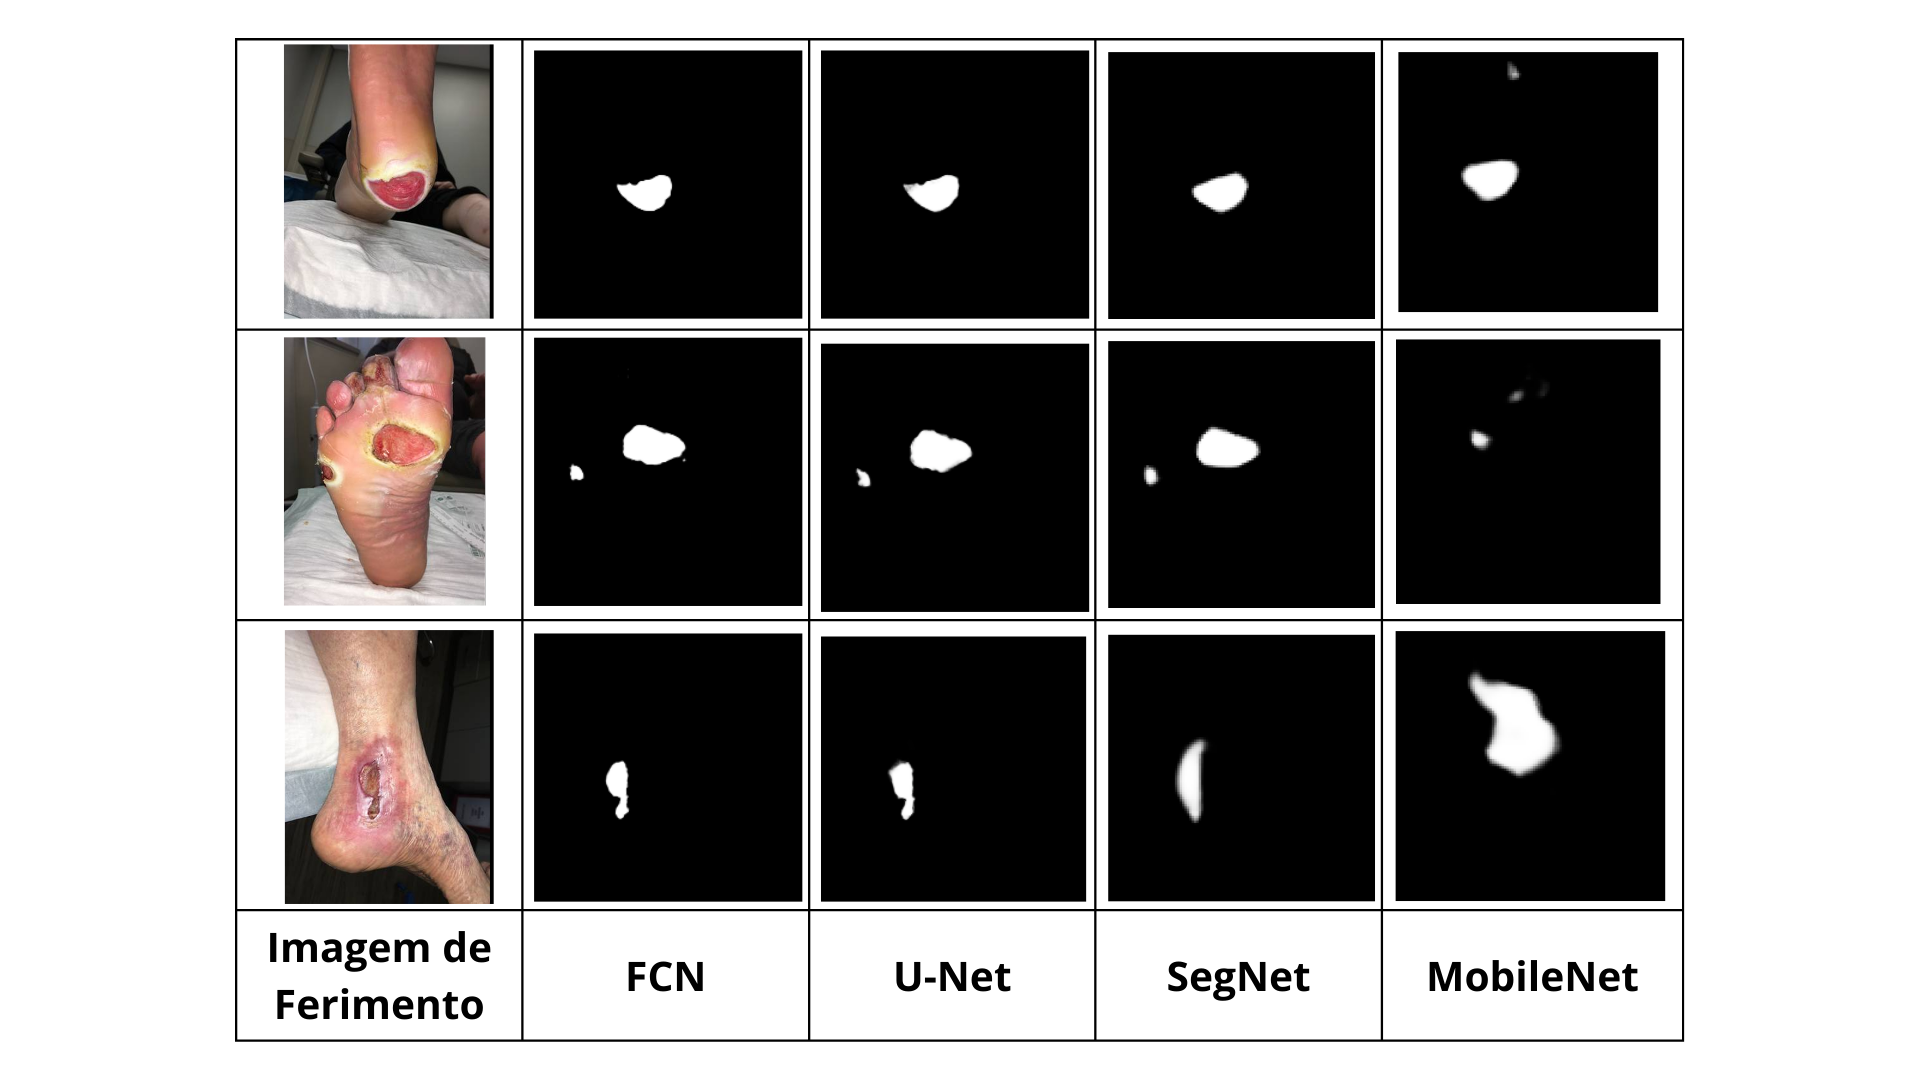
\includegraphics[width=0.9\textwidth]{img/resultado_segmentacao_modelos.png}
    \label{fig:resultSegmetationModels}
    \par\medskip\textbf{Fonte:} Autor
\end{figure}



Como podemos observa na segmentação de feridas malignas em imagens médicas revela diferenças notáveis em desempenho:

\textbf{\ac{FCN} e \ac{U-Net}:} Ambos os modelos se sobressaem com alta precisão, recall e coeficiente Dice, tornando-os escolhas eficazes para aplicações que exigem uma segmentação precisa das áreas afetadas.

\textbf{\ac{SegNet}:} Apresenta métricas ligeiramente inferiores, mas pode ser preferível em cenários com limitações computacionais devido à sua arquitetura menos complexa.

\textbf{\ac{MobileNetV2}:} Este modelo mostrou-se inadequado para a tarefa, evidenciando a necessidade de escolher cuidadosamente a arquitetura para aplicações clínicas críticas.

A escolha do modelo mais adequado para a segmentação de feridas malignas deve considerar as demandas específicas da aplicação clínica, incluindo objetivos, recursos disponíveis e a necessidade de precisão. Enquanto o \ac{FCN} e o \ac{U-Net} são recomendados para situações que exigem a máxima precisão, o \ac{SegNet} pode ser uma escolha eficiente em contextos com restrições de recursos.


\textbf{Conclusão:} Em última análise, a comparação entre esses modelos fornece uma base sólida para decisões informadas na segmentação de feridas malignas em imagens médicas, permitindo a escolha de uma abordagem que melhor atenda às necessidades específicas de cada caso clínico.

A comparação de Redes Neurais Convolucionais \ac{CNNs} avançadas com métodos tradicionais de análise de imagens médicas mostrou que as \ac{CNNs} tinham uma vantagem significativa na segmentação de feridas dolorosas. Modelos de aprendizagem profunda como \ac{U-Net}, \ac{FCN} e \ac{SegNet} demonstraram uma capacidade notável de reconhecer e diferenciar regiões de interesse com o mesmo grau de precisão ou superior aos métodos tradicionais.

As \ac{CNNs} têm benefícios distintos, um deles é a capacidade de reconhecer detalhes sutis e padrões complexos em imagens médicas; esses padrões são muitas vezes difíceis de reconhecer com abordagens manuais ou heurísticas. A capacidade das \ac{CNNs} de alterar seu comportamento dependendo do contexto clínico e do tipo de ferida, mantendo sua precisão, é indicativa de seu potencial na área médica como um todo.

Fatores como a capacidade de generalizar, a capacidade de aprender detalhes específicos sobre feridas dolorosas e a utilização de camadas especializadas como atenção e aumento de circunvoluções contribuíram para o sucesso das \ac{CNNs} em diversas situações clínicas. A versatilidade e a capacidade de aprender representações superiores de imagens médicas foram cruciais para a superioridade destes modelos sobre os métodos tradicionais, o que levou a uma maior capacidade de diagnosticar com precisão e rapidez as feridas que são malignas. \label{sec:perguntas}

\subsection{Contribuições e Perspectivas Futuras}

    Este estudo demonstra benefícios importantes no campo da oncologia da pele Isto tem contribuído para avanços no diagnóstico e monitoramento de feridas cancerígenas. Os resultados obtidos aprofundam a nossa compreensão do potencial da aprendizagem profunda na segmentação de imagens médicas, abrindo caminho para melhorar os modelos existentes e desenvolver novas arquiteturas.

    \textbf{Limitações e direções futuras:} Identificávamos limitações nos modelos existentes e sugiramos direções promissoras para pesquisas futuras. Uma delas é testar os modelos em diferentes condições para avaliar sua robustez. Além disso, recomenda-se a coleta de um conjunto maior de imagens em colaboração com instituições médicas para melhorar a generalização dos modelos.

    \textbf{Impacto na comunidade médica:} As ferramentas desenvolvidas neste estudo são de grande valor para a comunidade médica, pois facilitam a segmentação precisa de feridas malignos. Isso pode levar a diagnósticos mais precisos e tratamentos mais eficazes. As tendências futuras incluem a melhoria contínua da abordagem proposta. Expandir a aplicabilidade do modelo em uma gama mais ampla de situações clínicas. e explorar novos métodos de aprendizagem profunda. Para melhorar a segmentação de feridas cancerígenas.

    \textbf{Conclusão:} Em resumo, este estudo apresenta resultados promissores na segmentação de feridas oncológicas em imagens médicas. Esta é uma informação valiosa para pesquisas futuras. As contribuições deste estudo são notáveis para o avanço da medicina e as perspectivas futuras concentram-se na otimização contínua dos técnicos propostas e na exploração de novas abordagens de aprendizagem profunda para melhorar ainda mais a precisão da segmentação de feridas malignos.